\documentclass{article}

\usepackage{graphicx}
\usepackage{multirow}

\title{Note: Support Vector Machines}
\author{Sun Zhao}

\begin{document}
\maketitle
\newpage

\section{Support Vector Machines Intuition}
 A support vector machine(SVM for short) constructs a hyperplane or set of hyper-planes in a high- or infinite-dimensional space, which can be used for classification, regression, or other tasks. Intuitively, a good separation is achieved by the hyperplane that has the largest distance to the nearest training data point of any class (so-called functional margin), since in general the larger the margin the lower the generalization error of the classifier. $H_{1}, H_{2}, H_{3}$ in Fig. \ref{hyper-plane-example1} are three hypothesises trying to separate black and white pointers. Obviously, $H_{1}$ does not separate the classes. $H_{2}$ does, but only with a small margin. $H_{3}$ separates them with the maximum margin. SVM chooses the hyperplane so that the distance from it to the nearest data point on each side is maximized.
\begin{figure}[ht]
  \centering
  % Requires \usepackage{graphicx}
  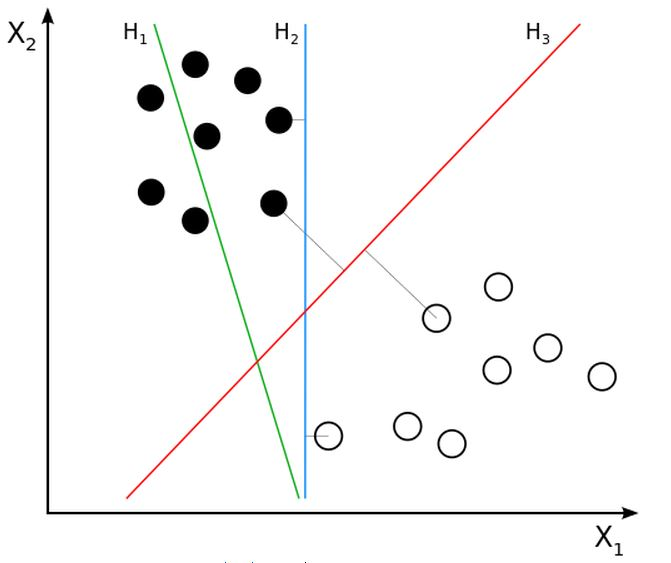
\includegraphics[width=5cm]{Figure1.jpg}\\
  \caption{}\label{hyper-plane-example1}
\end{figure}
 Recall that in logistic regression, we use $\Theta^{T}x = 0$ as the hyper-plane, and predict positive class if $\Theta^{T}x \ge 0$, otherwise, negative class. SVM is trying to keeps a minimum margin between the two classes and wants $\Theta^{T}x \ge 1$ if x is positive and $\Theta^{T}x \le -1$ if x is negative. Let $H_{1}$ denotes $\Theta^{T}x = 1$, $H_{0}$ denotes $\Theta^{T}x = -1$ and $H_{0}$ denotes $\Theta^{T}x = 0$. The margin distance between $H_{1}$ and $H_{-1}$ is $\frac{2}{||\Theta_{1 \ldots n}||}$ where $||\Theta_{1 \ldots n}||$ equals $\sqrt{\sum_{i = 1}^{n} \Theta_{i}^{2}}$. The location relationships between training examples and $H_{1}, H_{0}, H_{-1}$ is shown in Fig. \ref{hyper-plane-example2}. The optimization problem can be summarized as follow:\\
%Minimize $||\Theta_{1 \ldots n}||$\\
\begin{equation}
\min ||\Theta_{1 \ldots n}||
\end{equation}
Subject to(for any i = 1 $\ldots$ m)\\
\begin{equation}\label{}
y^{(i)}(\Theta^{T}x^{(i)}) \ge 1
\end{equation}
\begin{figure}[ht]
  \centering
  % Requires \usepackage{graphicx}
  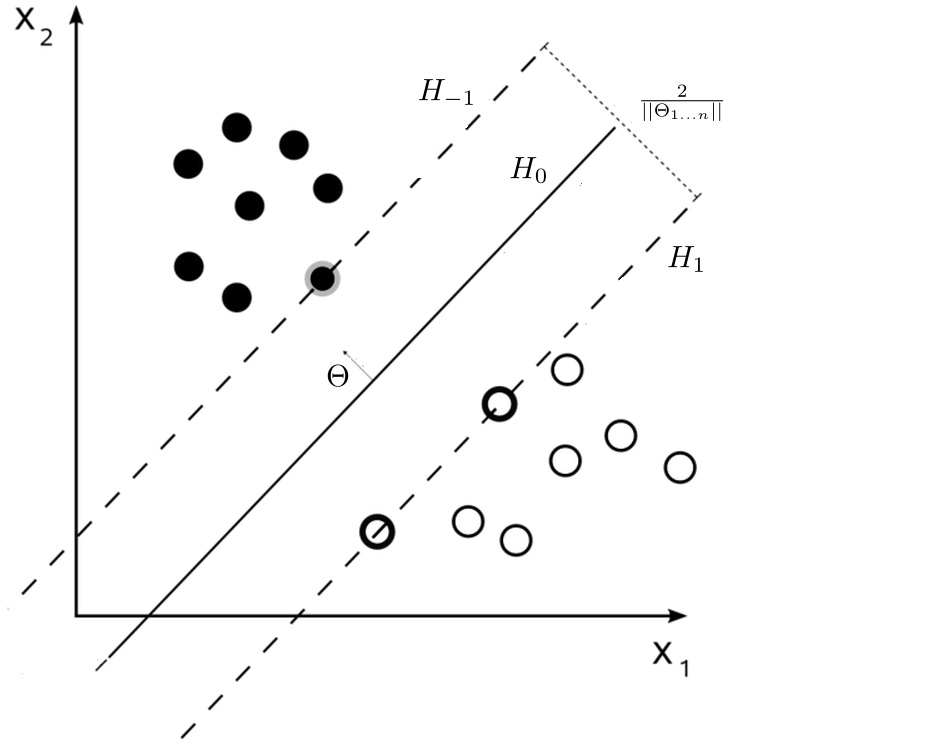
\includegraphics[width=5cm]{Figure2.jpg}\\
  \caption{}\label{hyper-plane-example2}
\end{figure}

\newpage
\section{Cost Function}
Instead of following the logarithm example cost function, SVM introduces cost function show in Fig. \ref{example_cost_funtion_visulization}. The new cost functions have following properties:
\begin{table}[h]
\begin{center}
\begin{tabular}{l}
if $y^{(i)}$=1, cost = 0 when $\Theta^{T}x^{(i)} \ge 1$\\
if $y^{(i)}$=0, cost = 1 when $\Theta^{T}x^{(i)} \le -1$\\
\end{tabular}
\end{center}
\end{table}
\begin{figure}[ht]
  \centering
  % Requires \usepackage{graphicx}
  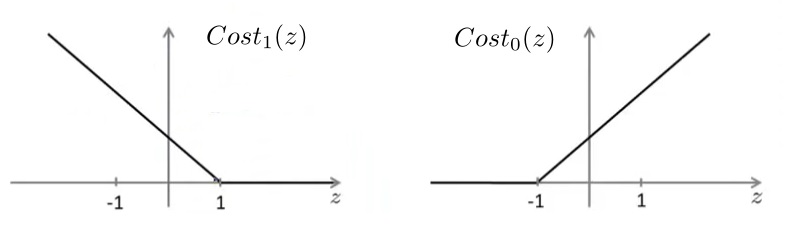
\includegraphics[width=10cm]{Figure3.jpg}\\
  \caption{}\label{example_cost_funtion_visulization}
\end{figure}
\end{document}
